\documentclass[a4paper,11pt]{jsarticle}


% 数式
\usepackage{amsmath,amsfonts}
\usepackage{bm}
\usepackage{physics}
% 画像
\usepackage[dvipdfmx]{graphicx}
% ローマ数字
\usepackage{otf}
% 単位
\usepackage{siunitx}
% 表
\usepackage{multirow}


\begin{document}

\title{機械学習概論 第1回レポート}
\author{05-211525 齋藤駿一}
\date{\today}
\maketitle

\section{交差検証}
まず,$p=1,2,\cdots, 10$のうちどれが最適なモデルかを考える.
ここでは,各$p$について前半の73年分(1876年1月~1948年12月)のデータを用いて10-foldの交差検証を行い,そのときの交差検証誤差を比較した.
その結果,交差検証誤差が最小となるのは$p=5$であることが分かった.

\begin{figure}[htbp]
  \centering
  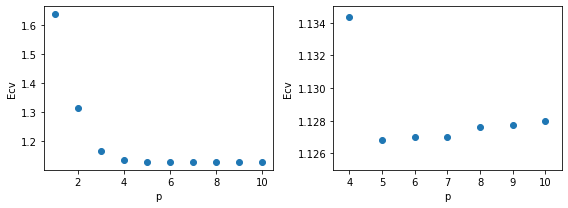
\includegraphics[width=10cm]{cv.png}
  \caption{10-foldの交差検証を行ったときの,$p$の値と交差検証誤差の関係.右図は左図を拡大したものであり,ここから交差検証誤差が最小となるのは$p=5$であることが読み取れる.}
  \label{fig:cv}
\end{figure}

\section{年平均気温の推定値の信頼区間(t-分布)}
ここでは,$p=5$として前半73年分のデータを学習し,後半の10年分(2012年~2021年)の各年について年平均気温を推定した.
また,その信頼区間を次の3つの方法で推定した.

\subsection{t-分布を仮定する方法}
まず,各データと回帰曲線の残差を正規分布に従う統計的に独立なノイズと仮定する.
このとき,73年分の訓練データを用いてその分散を推定することで,年平均気温の推定値はt-分布に従うと考えることができる.
そこで,各年の年平均気温の推定値に対して99\%信頼区間を求めると,次の表のようになった.

\begin{table}[htbp]
  \centering
  \caption{各年の年平均気温($\si{\degreeCelsius}$)の推定値の99\%信頼区間の上限と下限.PBはペアブートストラップ法,RBは残差ブートストラップ法を意味する.}
  \label{tab:99}
  \begin{tabular}{c|cccccc}
    年 & 下限(t-分布) & 上限(t-分布) & 下限(PB) & 上限(PB) & 下限(RB) & 上限(RB)\\
    \hline\hline
    2012 & 14.72 & 15.61 & 14.70 & 15.60 & 14.74 & 15.60\\
    2013 & 14.73 & 15.62 & 14.72 & 15.64 & 14.74 & 15.61\\
    2014 & 14.74 & 15.64 & 14.72 & 15.65 & 14.75 & 15.63\\
    2015 & 14.75 & 15.65 & 14.73 & 15.67 & 14.76 & 15.65\\
    2016 & 14.75 & 15.67 & 14.74 & 15.68 & 14.77 & 15.66\\
    2017 & 14.76 & 15.69 & 14.75 & 15.70 & 14.77 & 15.68\\
    2018 & 14.77 & 15.70 & 14.75 & 15.72 & 14.78 & 15.69\\
    2019 & 14.78 & 15.72 & 14.76 & 15.73 & 14.79 & 15.71\\
    2020 & 14.78 & 15.73 & 14.77 & 15.75 & 14.80 & 15.72\\
    2021 & 14.79 & 15.75 & 14.78 & 15.76 & 14.80 & 15.74\\
    \hline
  \end{tabular}
\end{table}

\subsection{ペアブートストラップ法}
同様のことをペアブートストラップ法で行った結果も同表に示す.

\subsection{残差ブートストラップ法}
同様のことを残差ブートストラップ法で行った結果も同表に示す.

\section{年平均気温の推定}
それぞれの方法で求めた信頼区間と,実際に観測された年平均気温を合わせてグラフにまとめると,次のようになる.
観測値がどれも推定値の信頼区間より上にあることから,東京の年平均気温は線形よりも急激に上昇していることが分かる.

\begin{figure}[htbp]
  \begin{minipage}[b]{0.32\linewidth}
    \centering
    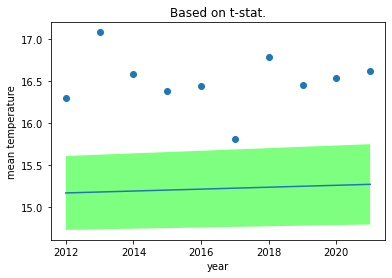
\includegraphics[width=\linewidth]{tstat.png}
    \caption{t-分布を仮定する方法}
  \end{minipage}
  \begin{minipage}[b]{0.32\linewidth}
    \centering
    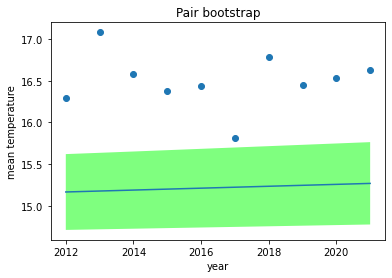
\includegraphics[width=\linewidth]{pair_bootstrap.png}
    \caption{ペアブートストラップ法}
  \end{minipage}
  \begin{minipage}[b]{0.32\linewidth}
    \centering
    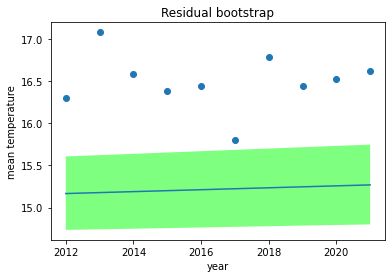
\includegraphics[width=\linewidth]{residual_bootstrap.png}
    \caption{残差ブートストラップ法}
  \end{minipage}
\end{figure}

\end{document}